\documentclass[11pt]{article}
\usepackage{graphicx}
%\usepackage{ngerman}
\usepackage[utf8x]{inputenc}
\usepackage{fancyvrb}
\usepackage{courier}
\usepackage{helvet}
\usepackage{tikz}
\usepackage{xcolor}
\usepackage{pdfpages}
\usetikzlibrary{calc}
\usepackage[strict]{changepage}
\usepackage{xspace}
\usepackage{hyperref}
\usepackage{cleveref}
\usetikzlibrary{shapes.geometric}
\usetikzlibrary{arrows}
\usetikzlibrary{positioning}
\usetikzlibrary{arrows.meta, automata, shapes, matrix,positioning}
\usepackage{amssymb}
\usepackage{pifont}% http://ctan.org/pkg/pifont
\usepackage{amsmath}
\usepackage{subcaption} 
\usepackage{float}
\usepackage{fixfoot}
\usepackage{graphicx}
\usepackage{wrapfig}
\usepackage{multicol}
\usepackage{listings}
\usepackage{fancyhdr} % Header
\usepackage[a4paper, total={15cm, 20cm}]{geometry} % Dimensions of the paper and the text area

% Other packages that might be useful in the future
%\usepackage{lingmacros}
%\usepackage{tree-dvips}
%\usepackage{ulem}
%\usepackage{amsthm}
%\usepackage{amsbsy}
%\usepackage{textcomp,gensymb}
%\usepackage{graphicx}
%\usepackage{mathtools}

% Custom variant of msc environment:
% - No "msc" keyword, longer partial messages
% - Increased vertical distance between messages
% - Less distance to the frame left and right
% - Less distance between header and processes
% - Less distance between footer and frame
% - Passing all given options down to the msc environment
\newenvironment{cmsc}[1][]{\msc[msc keyword={}, self message width=1.1cm, level height=0.6cm, environment distance=1.2cm, head top distance=0.75cm, foot distance=0.5cm, #1]}{\endmsc}

% No indentation at new paragraphs
\setlength{\parindent}{0pt}

% Distance between columns
\setlength{\columnsep}{1cm}
% Vertical line between columns
\setlength{\columnseprule}{0.5pt}
\def\columnseprulecolor{\color{gray}}

% Settings
\newcommand{\sheetNr}{}
\newcommand{\red}[1]{\color{red}#1\color{black}}
\newcommand{\loesung}{\color{green!50!black}Lösung:\color{black}\xspace}

%% Header
\fancyhf{}
\pagestyle{fancy}
\lhead{Installationsprobleme \sheetNr}
\setlength{\headheight}{40pt}

%% Automatic section titles
%\titleformat{\section}{\normalfont\Large\bfseries}{}{0em}{Exercise #1}
%\titleformat{\subsection}{\normalfont\large\bfseries}{}{0em}{#1)}

\begin{document}

\section{DeepDriving}
Das Beispiel aus dem Original-Paper von:\\
\url{http://deepdriving.cs.princeton.edu/}\\
muss 3 mal gedownloaded werden, weil die CheckSum nicht stimmt -.-'\\
und wenns funktionier kann mans nicht auspacken:\\
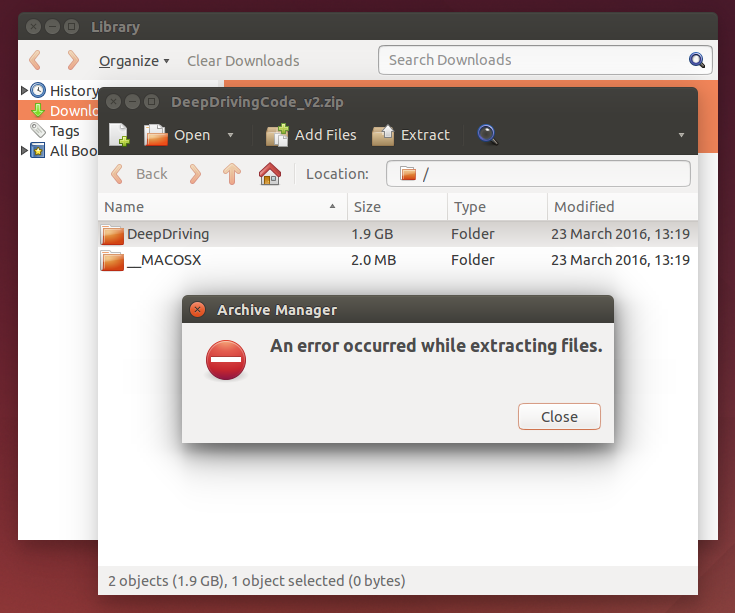
\includegraphics[scale=0.8]{cant-extract.PNG}

Installation nach Anleitung im ReadMe-File. 

Torcs läuft:\\
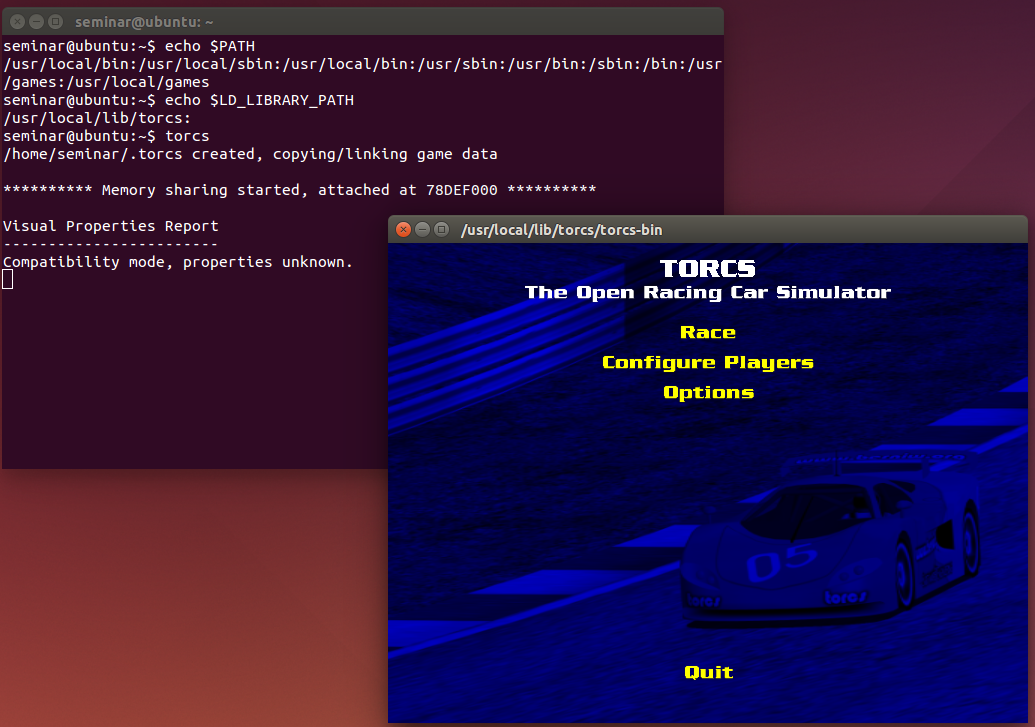
\includegraphics[scale=0.6]{torcs-proof.PNG}

Basierd darauf, dass die Grundlagen von Caffe funktionieren\\

Seltsam: Track-kopieren ist Punkt 3 und danach kommt Punkt 6?
\lstinputlisting[numbers=left, firstnumber = 47, basicstyle=\scriptsize,firstline=47, lastline=49]{ReadMe.txt}

Bei Punkt 6 funktioniert es nicht:\\
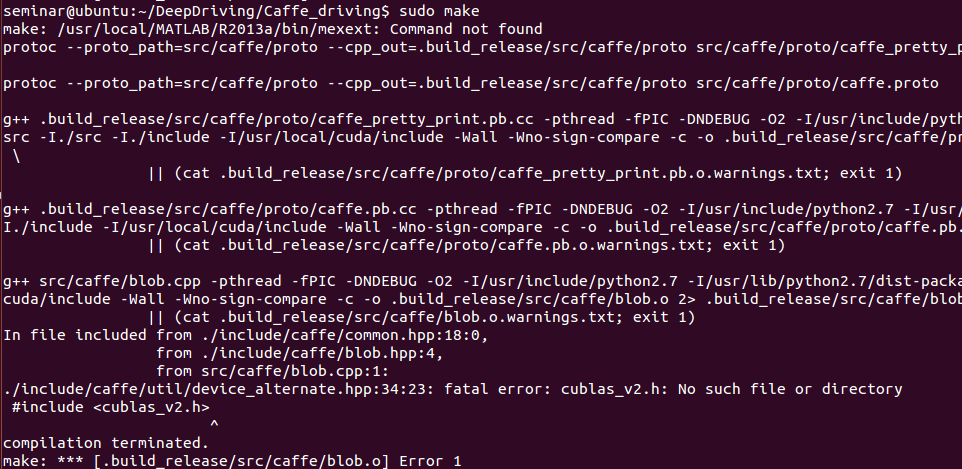
\includegraphics[scale=0.5]{caffe_driving-error1.PNG}\\
Er benötigt die \texttt{cublas\_v2.h} aus CUDA. Das geht aber nicht da ich (siehe 2) CUDA nicht installieren kann.
(\url{https://github.com/BVLC/caffe/issues/2704})

\section{Caffe} \label{Caffe}
	Originaler Versuch zu installieren hat Ubuntu zerschossen. Kann mich nicht einloggen ohne Absturz. Selbst bearbeiten der \texttt{.Xauthority} hilft nicht\\
	
	Die Grundlagen von Caffe wurden von hier entnommen:\\
	\url{http://caffe.berkeleyvision.org/install_apt.html}\\
	Abschnitt für 14.04
	
	Manche der folgenden Sachen werden nur alternativ gebraucht aber um alle Kombinationen zu testen installiere ich es trotzdem:
	\begin{itemize}
		\item CUDA:\\
			Nicht installierbar, da die VM kein Zugriff auf die GPU hat
		\item BLAS:
		\begin{lstlisting}
sudo apt-get install libopenblas-dev
		\end{lstlisting}
		\item ATLAS:
			\begin{lstlisting}
sudo apt-get install libatlas-base-dev
			\end{lstlisting}
	\end{itemize}
	
	Beim Makefile wurden die Optionen wie \texttt{CPU\_ONLY} angepasst\\
	
	Setze neu auf nach diesem Guide:\\
	\url{https://github.com/BVLC/caffe/wiki/Ubuntu-14.04-VirtualBox-VM}\\
		
	
\section{MontiSim}
	\begin{itemize}
		\item bei laufendem Server und RMIModel passiert nichts, wenn ich ein Szenario auswähle
		\item beim mobile-deploy: beim laden eines Szenarios, was auch in der Konsole geloggt wird, bekommt man nach ca. 2 Minuten einen Disconnect
	\end{itemize}
\section{CNNArchLang}
	Benutze das folgende Repo:\\
	\url{https://github.com/EmbeddedMontiArc/CNNArchLang}	
	
	\begin{enumerate}
		\item pom.xml:\\
			Die pom.xml funktioniert mittels
			\begin{lstlisting}
	mvn clean install --settings settings.xml
			\end{lstlisting}
			nur unter Windows aber nicht unter Ubuntu. Dann wird folgender Fehler geworfen:
			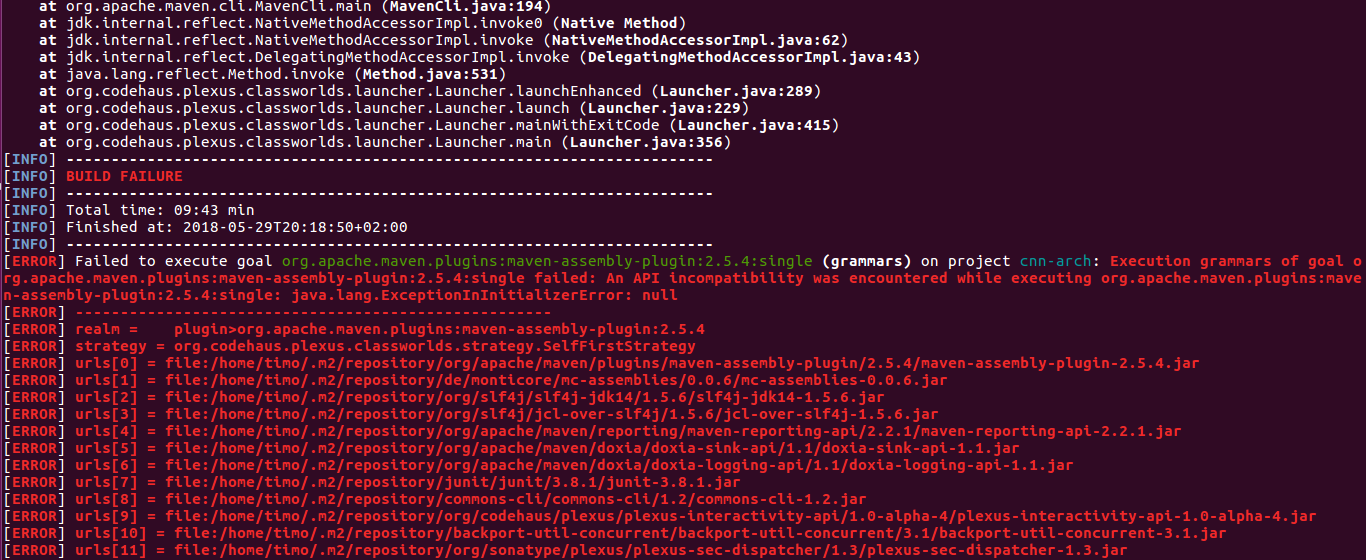
\includegraphics[scale=0.4]{CNNArchLang-Build-Failure.PNG}
			obwohl nichts was nicht benötigt war installiert wurde
		\item \texttt{import de.se\_rwth.commons.Joiners}:\\
			Nicht gefunden trotz maven build\\
			\loesung logging statt dem normalen commons paket nutzen
		\item \texttt{import javax.annotation.Nullable}:\\
		Auch nicht gefunden. \\
			\loesung
			\begin{lstlisting}
	<dependency>
		<groupId>com.google.code.findbugs</groupId>
		<artifactId>jsr305</artifactId>
		<version>3.0.2</version>
	</dependency>
			\end{lstlisting}
			im pom.xml
		\item \texttt{import freemarker.template.TemplateException}:\\	
			fehlt auch.\\
			\loesung manuelles Installieren via IntelliJ $\rightarrow$ libs $\rightarrow$ Maven
		\item keinerlei Informationen wie man ein Beispiel-Netz benutzt. Nur die Tests, welche ohne Kommentare wenig helfen
			In etwa so?
			\begin{lstlisting}[language=java, numbers=left, basicstyle=\scriptsize]
Scope symTab = createSymTab("src/test/resources/architectures");
CNNArchCompilationUnitSymbol a = symTab.<CNNArchCompilationUnitSymbol>resolve(
                                         "Alexnet",
CNNArchCompilationUnitSymbol.KIND).orElse(null);
			\end{lstlisting}
		\item es laufen manche Tests nicht durch:
			\begin{itemize}
				\item \texttt{GeneratorTest.java}:\\
					\begin{figure}[H]
						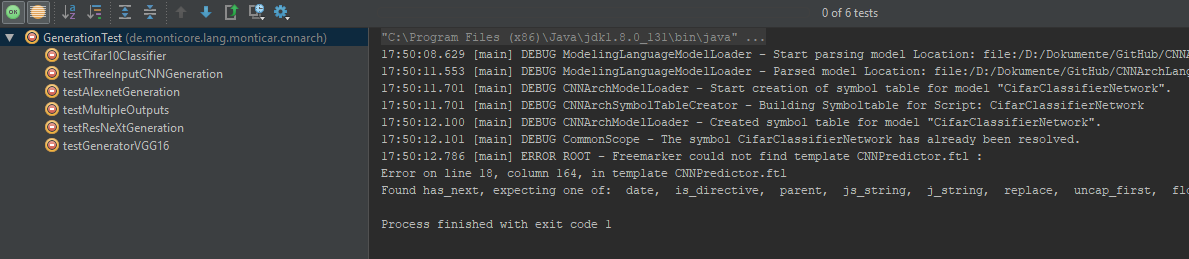
\includegraphics[scale=0.5]{CNNArchLang-generationTest.PNG}
					\end{figure}
					
					(vollständige Fehlermeldung in \texttt{GenerationTest-errormsg.txt})
					Freemaker scheint ein Problem zuhaben. Hängt vielleicht mit Punkt 4 zusammen
				\item (Rest gefixt)
			\end{itemize}
				
	\end{enumerate}	
\end{document}
